\documentclass{beamer}

\usepackage[utf8]{inputenc}
\usepackage[T1]{fontenc}
\usepackage[francais]{babel}
\usetheme{Madrid}


\title{Comparatif des performances d’une application en fonction des paramètres de compilation utilisés et analyse des performances }

\subtitle{TER M1 Informatique}

\author{Pierre \textsc{Tassel} sous la direction de Sid \textsc{Touati}}

\institute[Universitée Nice Sophia Antipolis] 
{Département Informatique\\
Universitée Nice Sophia Antipolis
\and
Master Informatique}

\date{\today}

\subject{Présentation TER}

% Let's get started
\begin{document}

\begin{frame}
  \titlepage
\end{frame}

\begin{frame}{Plan}
  \tableofcontents
  % You might wish to add the option [pausesections]
\end{frame}

% Section and subsections will appear in the presentation overview
% and table of contents.
\section{Présentation du programme}

\begin{frame}{Présentation du programme}{MinMax et le jeux de l'Awale}
\begin{itemize}
  \item
    MinMax avec coupes Alpha Beta
  \item
    Variante du jeux de l'Awale avec 6 cases et 4 graines par case
  \item
    Ecrit en C++ par M \textsc{Régin}
  \end{itemize}
  \begin{figure}
   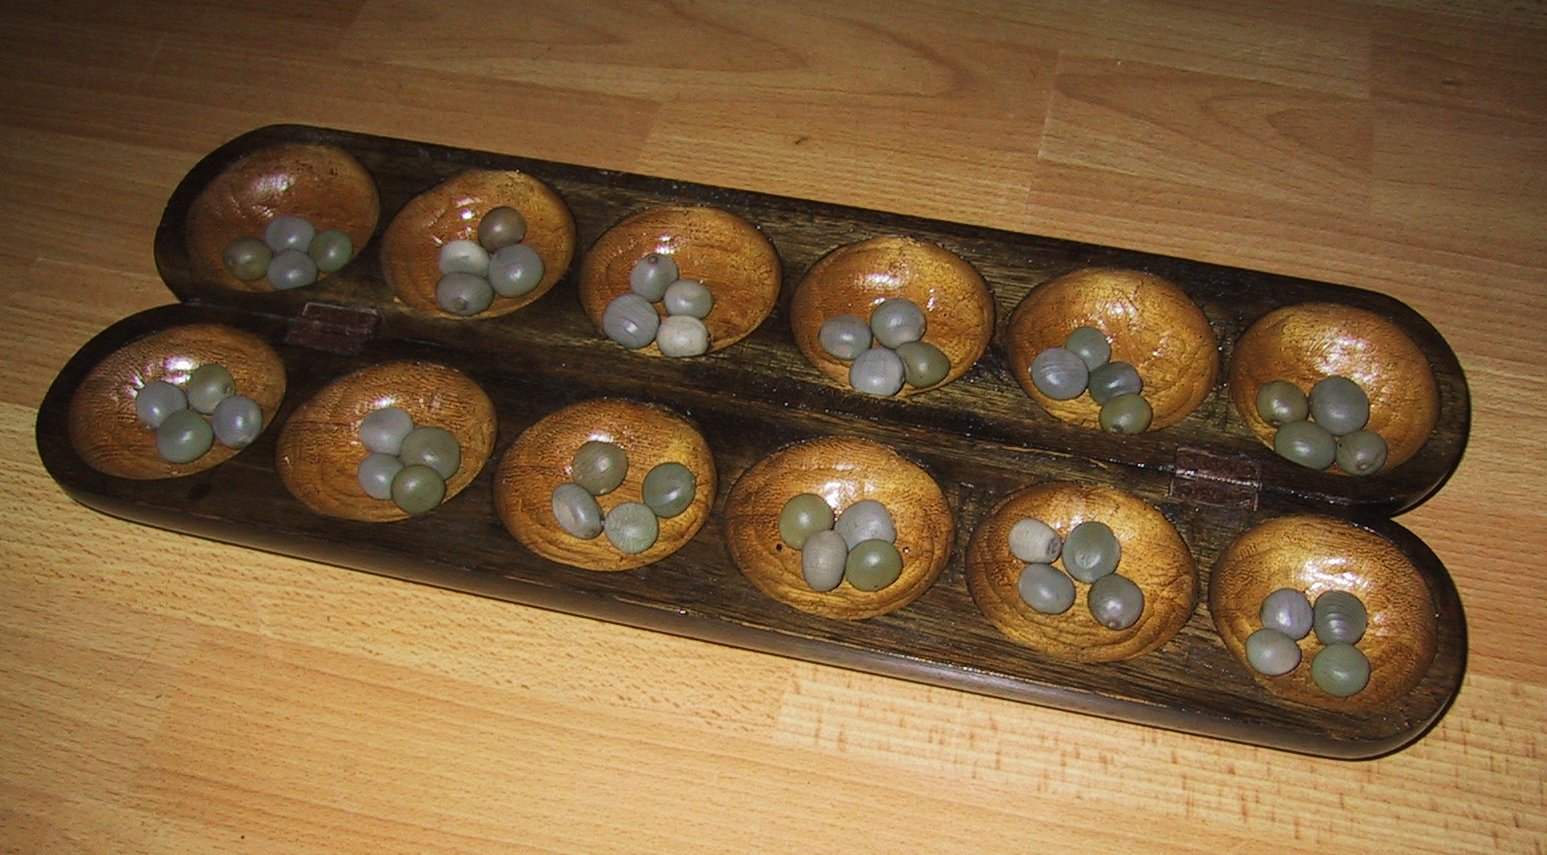
\includegraphics[width= 0.7\linewidth, keepaspectratio]{Awale.jpg}
   \caption{Le jeu de l'Awalé.\label{Fig:awale}}
\end{figure}
\end{frame}

\section{Démarche expérimentale}
\begin{frame}{Démarche expérimentale}{Environnement matériel et logiciel}
\begin{itemize}
  \item
  	Processeur Scaling désactivé, processeur 8 coeurs 2,5GHz, 8Go DDR3, 250Go de SSD
  \item
    Environnement minimaliste en CLI, Arch Linux basé sur noyau 4.14.13-1
    \item
    3 compilateurs analysés, GCC, ICC et CLang dernières versions disponible
    \item
    Fichier d'entrée généré en faisant jouer le programme contre lui même
    \item
    On répète les exécutions 20 fois pour chaque configurations testé
\end{itemize}
\end{frame}

\section{Analyse des performances séquentielles}

\begin{frame}{Analyse des performances séquentielles}

\begin{figure}
	\begin{columns}
      \column{.3\linewidth}
      \caption{Temps d’exécution séquentiel quand le programme commence.}
      \label{fig:exec_seq}
      \column{.6\linewidth}
      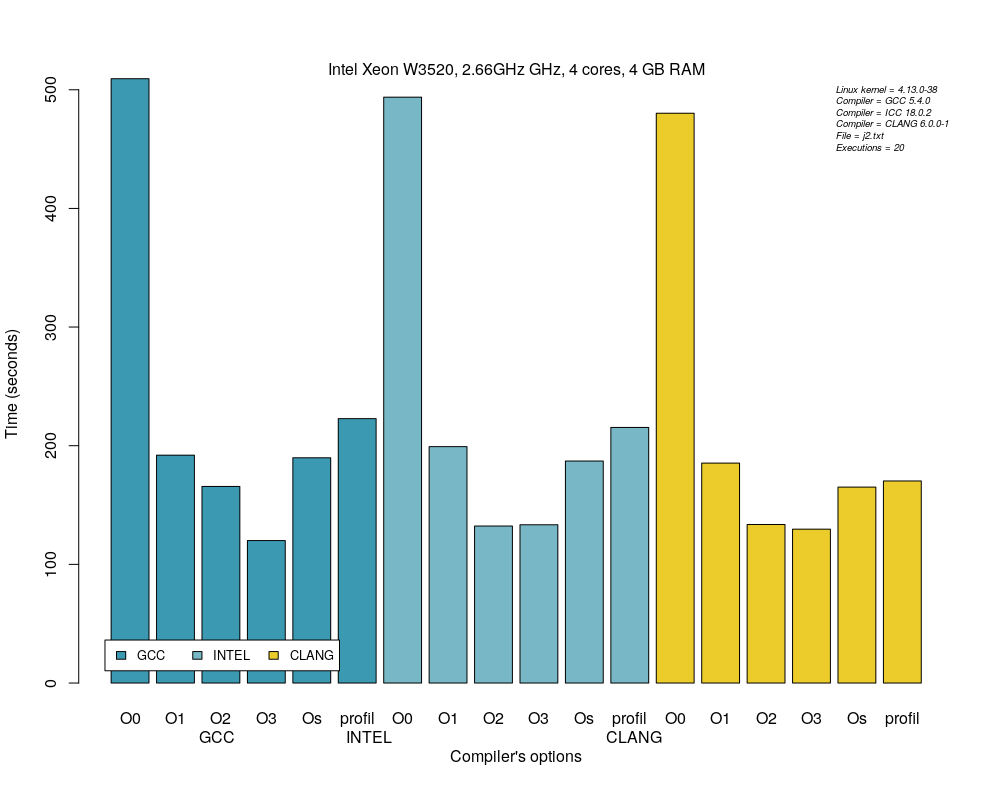
\includegraphics[width=\textwidth]{GCCvsICCvsCLANG_j2.png}
    \end{columns}
\end{figure}
\end{frame}

\section{Profilage du code}

\subsection{GProf}
\begin{frame}{Profilage du code}{GProf}
\begin{figure}
        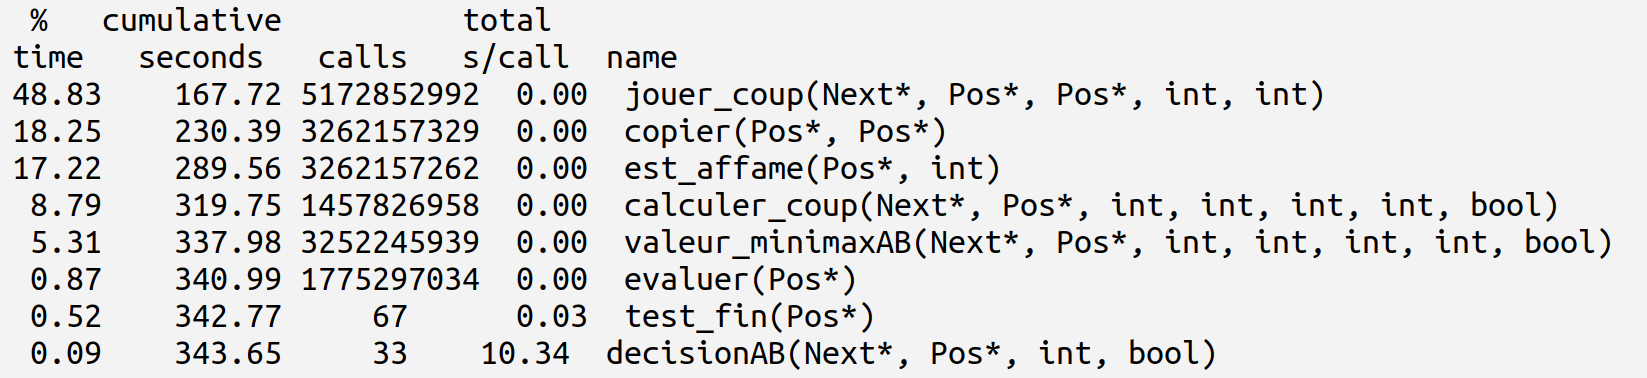
\includegraphics[width=\textwidth]{gprof.png}
        \caption{Analyse du code avec GProf.\label{Fig:GProf}}
\end{figure}
\end{frame}

\subsection{vTune}
\begin{frame}{Profilage du code}{vTune}
\begin{columns}
    \column{6.5cm}
    \begin{figure}
      \centering
   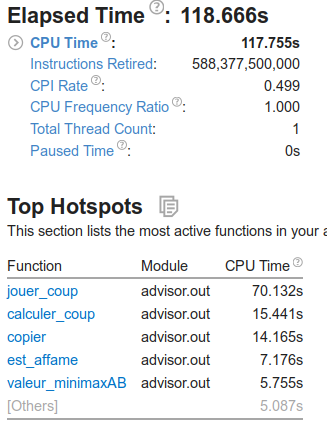
\includegraphics[width=0.75\textwidth]{vtune.png}
   \caption{vTune analyse usage processeur.\label{Fig:vTune_proc}}
    \end{figure}
    \column{6.5cm}
    \begin{figure}
      \centering
   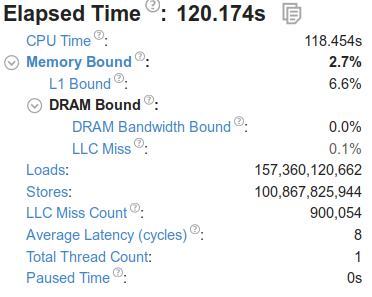
\includegraphics[width=0.9\textwidth]{memory_vtune.png}
   \caption{vTune analyse usage mémoire.\label{Fig:vTune_mem}}
    \end{figure}
    
  \end{columns}
\end{frame}

\section{Difficultés de l'optimisation du code}

\begin{frame}{Difficultés de l'optimisation du code}
\begin{itemize}
\item
Algorithme très séquentiel
\item
Nombre d'itérations faibles
\item
Usage de pointeurs qui pourraient aveugler les compilateurs
\end{itemize}
\end{frame}

\section{Parallélisme de donnée}

\subsection{Approche naïve}
\begin{frame}{Approche naïve}
	\begin{figure}

	\begin{columns}
      \column{.25\linewidth}
      \caption{Résultat ajout parallélisme avec compilateur Intel.\label{Fig:naif_intel}}
      \column{.72\linewidth}
      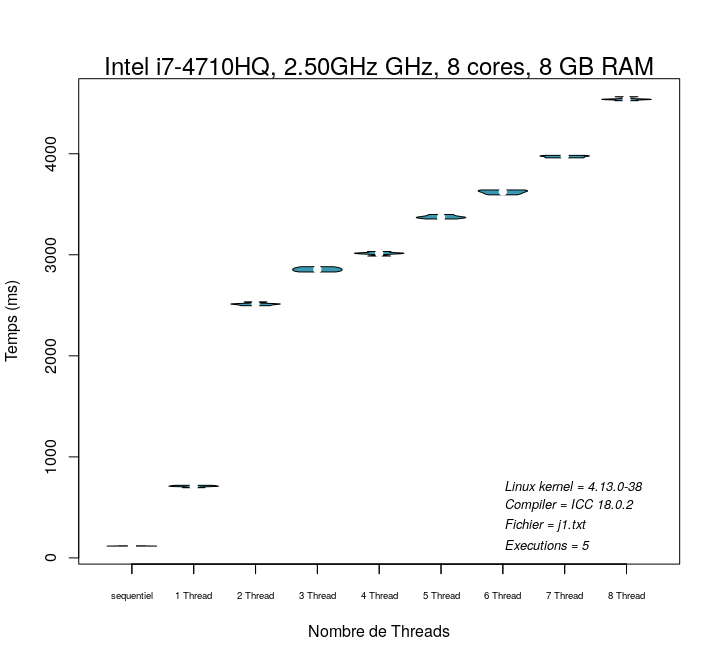
\includegraphics[width=\textwidth]{intel_parallel_naif.png}
    \end{columns}	
   		
	\end{figure}
\end{frame}

\subsection{False Sharing}
\begin{frame}{False Sharing}
	\begin{figure}
	\begin{columns}
      \column{.72\linewidth}
      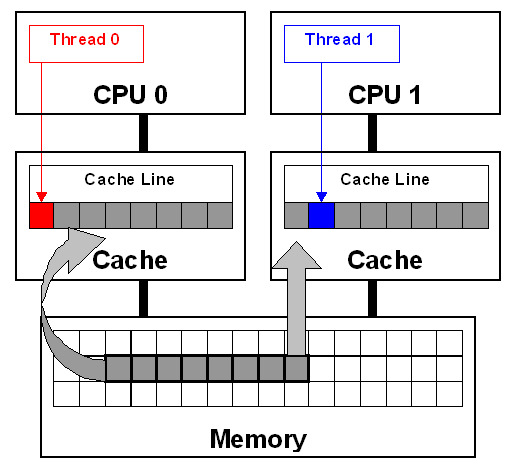
\includegraphics[width=\textwidth]{false_sharing.jpg}
      \column{.25\linewidth}
      \caption{Le phénomène de False Sharing.\label{Fig:false_sharing}}
    \end{columns}	
    \end{figure}
\end{frame}

\subsection{Thread Affinity}
\begin{frame}{Thread Affinity}
	\begin{figure}
	\begin{columns}
      \column{.25\linewidth}
      \caption{Analyse de l'impact du placement des threads.\label{Fig:thread_affinity}}
      \column{.72\linewidth}
      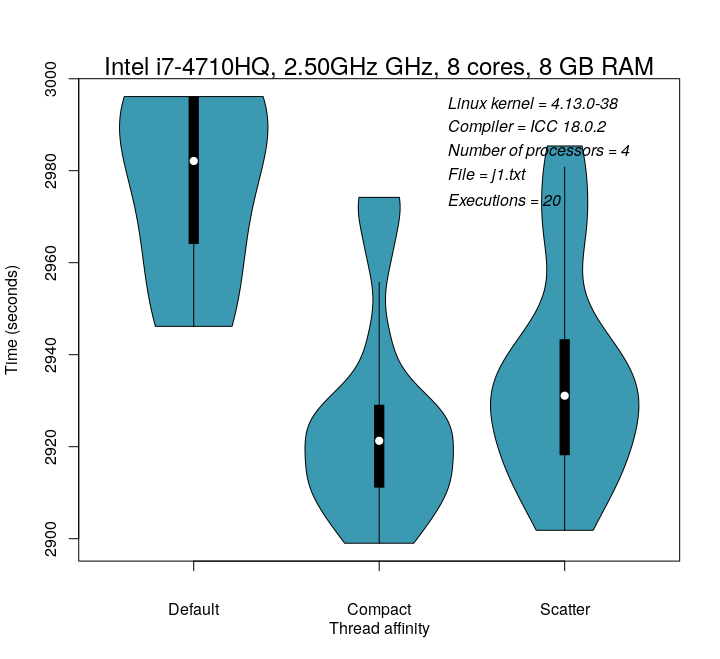
\includegraphics[width=\textwidth]{defaultVSscatterVScompact.png}
    \end{columns}	
	\end{figure}
\end{frame}

\subsection{Utilisation outils Intel}

\begin{frame}{Intel Advisor}
	\begin{figure}
	\begin{columns}
      \column{.60\linewidth}
      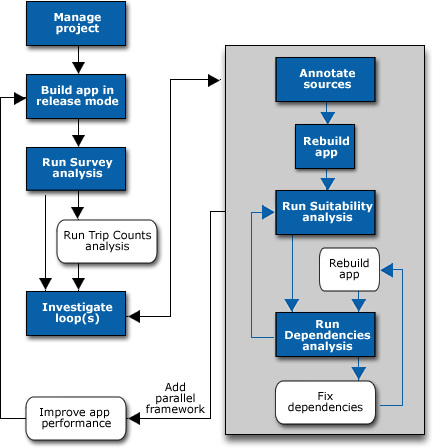
\includegraphics[width=\textwidth]{Intel.jpg}
      \column{.25\linewidth}
      \caption{Processus itératif d'Intel pour ajout parallélisme.\label{Fig:intel_iter}}
    \end{columns}	
    \end{figure}
\end{frame}

\section{Modification Algorithmique}


\begin{frame}{Modification Algorithmique}

\begin{itemize}
  \item
    Dictionnaires ouvertures.
  \item
    Trie des coups.
  \item
    Table de transposition.
 \end{itemize}	
\end{frame}


\subsection{Trie coups}

\begin{frame}{Trie coups}
	\begin{figure}
	\begin{columns}
      \column{.25\linewidth}
      \caption{Analyse de l'impact du trie des coups.\label{Fig:trie}}
      \column{.72\linewidth}
      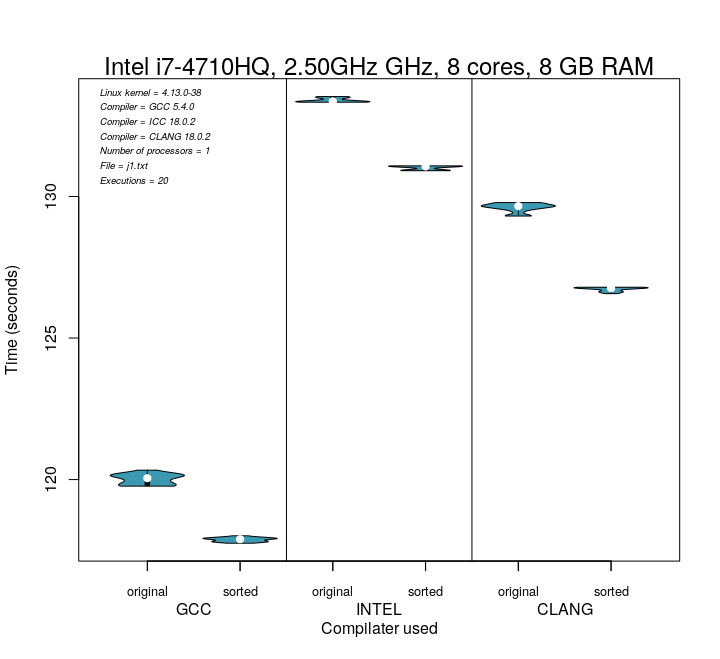
\includegraphics[width=\textwidth]{trie.png}
    \end{columns}	
	\end{figure}
\end{frame}

\subsection{Table de transposition}

\begin{frame}{Table de transposition}
	\begin{figure}
	\begin{columns}
      \column{.5\linewidth}
      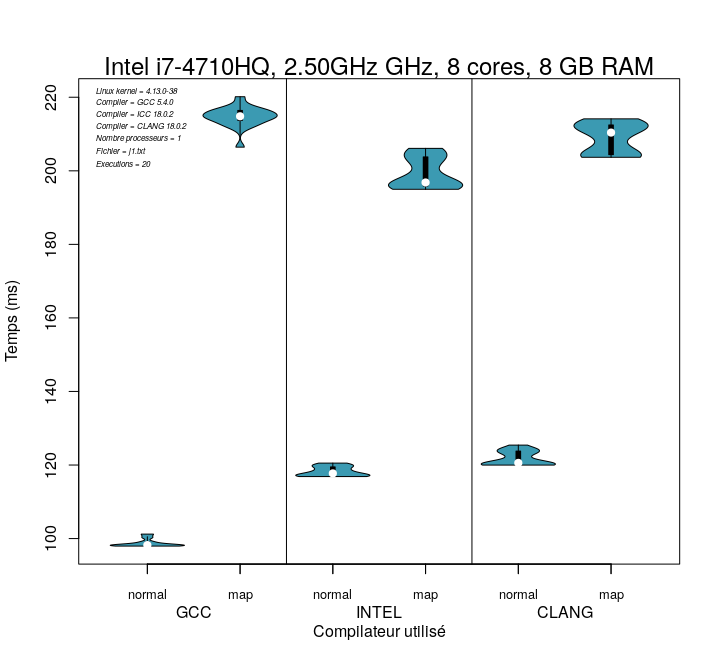
\includegraphics[width=\textwidth]{sorted_map.png}
      \caption{Arbre binaire de recherche.\label{Fig:arbre_binaire}}
      \column{.5\linewidth}
      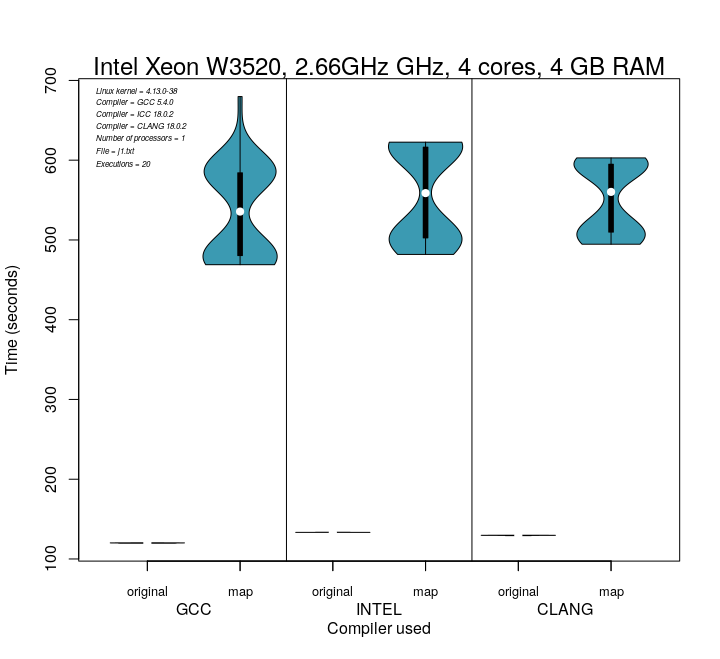
\includegraphics[width=\textwidth]{unsorted_map.png}
      \caption{Table de hashage.\label{Fig:arbre_binaire}}
    \end{columns}	
	\end{figure}
\end{frame}

\section{Conclusion}

\begin{frame}{Conclusion et perspective}
\begin{itemize}
  \item
    Dictionnaires ouvertures.
  \item
    Trie des coups.
  \item
    Table de transposition.
 \end{itemize}	
\end{frame}


\end{document}


